\documentclass[11pt,a4paper]{article}
\usepackage[T1]{fontenc}
\usepackage{lmodern}
\usepackage[margin=2.1cm]{geometry}
\usepackage{amsmath,amssymb}
\usepackage{microtype}
\usepackage{tikz}
\usepackage{booktabs}
\usepackage{float}
\usepackage{url}
\usepackage[hidelinks]{hyperref}
\newcommand{\Z}{\mathbb Z}
\newcommand{\Snaky}{S}
\newcommand{\paper}{\emph{Snaky in 21 Maker moves}}
\setlength{\parskip}{3.5pt}
\setlength{\parindent}{0pt}
\newcommand{\head}[1]{\vspace{4pt}\noindent\textbf{#1}\quad}

\begin{document}

\begin{center}
{\LARGE\bfseries A companion to \emph{Snaky in 21 Maker moves}}\\[6pt]
{\large how the proof works, in figures}\\[8pt]
{\small OpenAI, \emph{Snaky in 21 Maker moves}, 25 September 2026\\
\url{https://github.com/openai/math/tree/main/preprints/Snaky-in-21-Maker-moves-September-25-2026}}
\end{center}

\vspace{-4pt}

This companion follows the preprint \paper{} and supplies the pictures its text
implies but does not draw: the combination rule as a diagram, the certificate as
a whole, the last card, and one play. It is not needed to check the proof, and it
changes nothing in the paper: every numbered reference below --- Definition~2,
Lemma~3, Proposition~5, Section~4 --- is to the paper as published. Section~7
says how the figures and the small computational claims in this text were
produced.

\section{The game, the claim, the shape}

Maker and Breaker alternately claim one cell of $\Z^2$, Maker first, and ownership
is permanent. Maker wins as soon as its cells contain a copy of
\[
\Snaky=\{(0,0),(1,0),(2,0),(3,0),(3,1),(4,1)\}
\]
under any translation, reflection or quarter turn; Breaker need never build
anything itself. The theorem is that one Maker policy wins against every legal
Breaker play within $21$ Maker claims. Corollary~6 sharpens the board as well:
the same policy confines its claims to a fixed set of $251$ cells, so the game is
already won on a $17\times17$ square.

The quantifiers matter, because the paper proves $\exists\sigma\,\forall\beta$ and
nothing weaker: the policy $\sigma$ is fixed in advance, and the bound holds for
every sequence $\beta$ of legal Breaker replies, including replies the policy
never anticipated. Everything below is in service of that order of quantifiers.

% ---------------------------------------------------------------------------
%  Generated by gen_tikz.py; edit that, not this.
% ---------------------------------------------------------------------------
\begin{figure}[H]
\centering
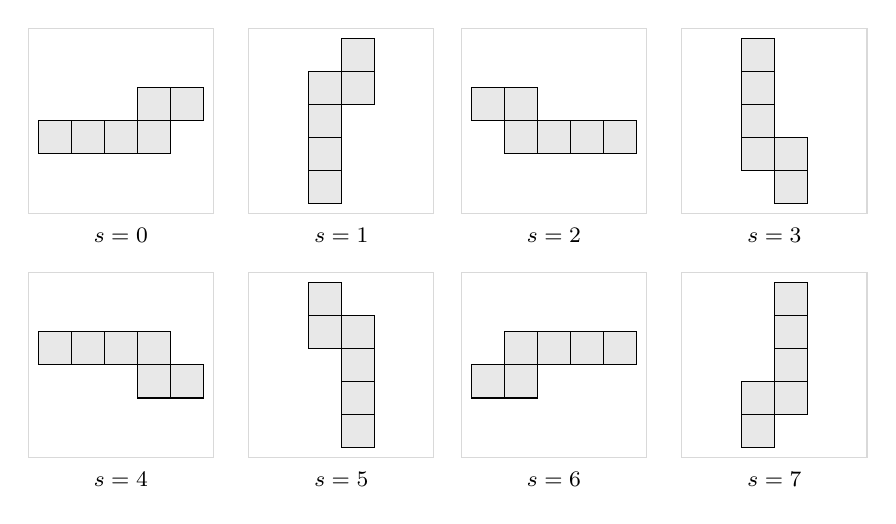
\begin{tikzpicture}[x=4.2mm,y=4.2mm,font=\small]
\begin{scope}[xshift=0.0cm,yshift=0.0cm]
\draw[gray!30] (0,0) rectangle (5.6,5.6);
\filldraw[fill=gray!18] (0.30,1.80) rectangle +(1,1);
\filldraw[fill=gray!18] (1.30,1.80) rectangle +(1,1);
\filldraw[fill=gray!18] (2.30,1.80) rectangle +(1,1);
\filldraw[fill=gray!18] (3.30,1.80) rectangle +(1,1);
\filldraw[fill=gray!18] (3.30,2.80) rectangle +(1,1);
\filldraw[fill=gray!18] (4.30,2.80) rectangle +(1,1);
\node[below,font=\footnotesize] at (2.8,-.15) {$s=0$};
\end{scope}
\begin{scope}[xshift=2.8cm,yshift=0.0cm]
\draw[gray!30] (0,0) rectangle (5.6,5.6);
\filldraw[fill=gray!18] (1.80,0.30) rectangle +(1,1);
\filldraw[fill=gray!18] (1.80,1.30) rectangle +(1,1);
\filldraw[fill=gray!18] (1.80,2.30) rectangle +(1,1);
\filldraw[fill=gray!18] (1.80,3.30) rectangle +(1,1);
\filldraw[fill=gray!18] (2.80,3.30) rectangle +(1,1);
\filldraw[fill=gray!18] (2.80,4.30) rectangle +(1,1);
\node[below,font=\footnotesize] at (2.8,-.15) {$s=1$};
\end{scope}
\begin{scope}[xshift=5.5cm,yshift=0.0cm]
\draw[gray!30] (0,0) rectangle (5.6,5.6);
\filldraw[fill=gray!18] (0.30,2.80) rectangle +(1,1);
\filldraw[fill=gray!18] (1.30,1.80) rectangle +(1,1);
\filldraw[fill=gray!18] (1.30,2.80) rectangle +(1,1);
\filldraw[fill=gray!18] (2.30,1.80) rectangle +(1,1);
\filldraw[fill=gray!18] (3.30,1.80) rectangle +(1,1);
\filldraw[fill=gray!18] (4.30,1.80) rectangle +(1,1);
\node[below,font=\footnotesize] at (2.8,-.15) {$s=2$};
\end{scope}
\begin{scope}[xshift=8.3cm,yshift=0.0cm]
\draw[gray!30] (0,0) rectangle (5.6,5.6);
\filldraw[fill=gray!18] (1.80,1.30) rectangle +(1,1);
\filldraw[fill=gray!18] (1.80,2.30) rectangle +(1,1);
\filldraw[fill=gray!18] (1.80,3.30) rectangle +(1,1);
\filldraw[fill=gray!18] (1.80,4.30) rectangle +(1,1);
\filldraw[fill=gray!18] (2.80,0.30) rectangle +(1,1);
\filldraw[fill=gray!18] (2.80,1.30) rectangle +(1,1);
\node[below,font=\footnotesize] at (2.8,-.15) {$s=3$};
\end{scope}
\begin{scope}[xshift=0.0cm,yshift=-3.1cm]
\draw[gray!30] (0,0) rectangle (5.6,5.6);
\filldraw[fill=gray!18] (0.30,2.80) rectangle +(1,1);
\filldraw[fill=gray!18] (1.30,2.80) rectangle +(1,1);
\filldraw[fill=gray!18] (2.30,2.80) rectangle +(1,1);
\filldraw[fill=gray!18] (3.30,1.80) rectangle +(1,1);
\filldraw[fill=gray!18] (3.30,2.80) rectangle +(1,1);
\filldraw[fill=gray!18] (4.30,1.80) rectangle +(1,1);
\node[below,font=\footnotesize] at (2.8,-.15) {$s=4$};
\end{scope}
\begin{scope}[xshift=2.8cm,yshift=-3.1cm]
\draw[gray!30] (0,0) rectangle (5.6,5.6);
\filldraw[fill=gray!18] (1.80,3.30) rectangle +(1,1);
\filldraw[fill=gray!18] (1.80,4.30) rectangle +(1,1);
\filldraw[fill=gray!18] (2.80,0.30) rectangle +(1,1);
\filldraw[fill=gray!18] (2.80,1.30) rectangle +(1,1);
\filldraw[fill=gray!18] (2.80,2.30) rectangle +(1,1);
\filldraw[fill=gray!18] (2.80,3.30) rectangle +(1,1);
\node[below,font=\footnotesize] at (2.8,-.15) {$s=5$};
\end{scope}
\begin{scope}[xshift=5.5cm,yshift=-3.1cm]
\draw[gray!30] (0,0) rectangle (5.6,5.6);
\filldraw[fill=gray!18] (0.30,1.80) rectangle +(1,1);
\filldraw[fill=gray!18] (1.30,1.80) rectangle +(1,1);
\filldraw[fill=gray!18] (1.30,2.80) rectangle +(1,1);
\filldraw[fill=gray!18] (2.30,2.80) rectangle +(1,1);
\filldraw[fill=gray!18] (3.30,2.80) rectangle +(1,1);
\filldraw[fill=gray!18] (4.30,2.80) rectangle +(1,1);
\node[below,font=\footnotesize] at (2.8,-.15) {$s=6$};
\end{scope}
\begin{scope}[xshift=8.3cm,yshift=-3.1cm]
\draw[gray!30] (0,0) rectangle (5.6,5.6);
\filldraw[fill=gray!18] (1.80,0.30) rectangle +(1,1);
\filldraw[fill=gray!18] (1.80,1.30) rectangle +(1,1);
\filldraw[fill=gray!18] (2.80,1.30) rectangle +(1,1);
\filldraw[fill=gray!18] (2.80,2.30) rectangle +(1,1);
\filldraw[fill=gray!18] (2.80,3.30) rectangle +(1,1);
\filldraw[fill=gray!18] (2.80,4.30) rectangle +(1,1);
\node[below,font=\footnotesize] at (2.8,-.15) {$s=7$};
\end{scope}
\end{tikzpicture}
\caption{The target in its eight allowed orientations, in the codes
$s=0,\dots,7$ that the certificate data use: $s=0$ is $(x,y)$, then $s=1,2,3,4,5,
6,7$ apply $(y,x)$, $(-x,y)$, $(y,-x)$, $(x,-y)$, $(-y,x)$, $(-x,-y)$, $(-y,-x)$.
Every translate of any one of them is a win, so a Maker policy may choose its
orientation in advance and change it later.}
\label{fig:target}
\end{figure}


\section{Cards: the only objects the proof uses}

The paper never reasons about a position directly. It reasons about a
\emph{card}, a triple $(A,T,h)$ of finite sets $A\subseteq T\subset\Z^2$ and an
integer $h\ge1$, which is a promise:

\begin{quote}
at every position with Maker to move at which Maker owns $A$ and Breaker owns
nothing in $T$, Maker has already completed a copy or can complete one within $h$
further Maker claims.
\end{quote}

This is Definition~2 of the paper, and three features of it do all the work.
First, it constrains only $A$ and $T$: extra Maker cells are free, and Breaker
cells outside $T$ are irrelevant. Second, it says nothing about how the position
was reached --- no assumption on the sizes of $M$ and $B$, no assumption that the
cells of $A$ were claimed consecutively, or that they are near each other. Third,
it counts only \emph{future} Maker claims. A card is therefore portable: any
placement $F$ --- a signed permutation of the coordinates followed by a
translation, one of the eight of Figure~1 --- carries a valid card to a valid one
with the same height.

The paper's figures are all of this kind: dots for the cells that must already be
Maker's, a small square for the next cell to claim, circles or crosses for the
cells the argument turns on.

\section{The one step: combining at a pivot}\label{sec:pivot}

Every one of the $722$ numbered lines of the certificate is a single application
of one lemma. Lemma~3 of the paper: given valid claims $(A_i,T_i,h_i)$,
$1\le i\le r$, and a cell $p$, the triple below --- equation~(2) of the paper,
numbered~(1) here --- is again a valid claim, where
\begin{equation}\label{eq:combination}
T=\{p\}\cup\bigcup_{i=1}^{r}T_i,\qquad
A=\Big(\bigcup_{i=1}^{r}A_i\ \cup\ \bigcap_{i=1}^{r}T_i\Big)\setminus\{p\},
\qquad h=1+\max_i h_i .
\end{equation}
Why: Maker claims $p$ (if $p$ is already Maker's, any free cell instead --- a real
move, and it is counted). Because $p\in T$ and Breaker avoids $T$, Breaker does
not own $p$. After that single claim Maker owns every $A_i$ and the whole common
part $\bigcap_iT_i$, so \eqref{eq:combination} holds. Breaker's one reply $b$
cannot lie in every $T_i$, since it is not in their intersection; choose a child
with $b\notin T_i$, and the older Breaker stones avoid $T_i$ because
$T_i\subseteq T$. That child is intact and delivers the win in $h_i\le h-1$
further claims. One stone, one surviving child: this is the whole mechanism.

\head{What a pivot is.} The paper names $p$ the \emph{pivot} from Section~3
onwards --- the data carry ``a pivot coordinate'' per line, Table~1 records that
all the children's requirements become ``the pivot'', and Section~4 has Maker
``claim its placed pivot $F(p)$'' --- but the lemma itself only says
``let $p\in\Z^2$''. The usage is uniform
enough to define:

\begin{quote}
\textbf{Definition (pivot; reconstruction).} Let $(A_i,T_i,h_i)$, $1\le i\le r$,
be valid claims and $p\in\Z^2$. In an application of \eqref{eq:combination} the
cell $p$ is the \emph{pivot} of the application and $(A,T,h)$ is the
\emph{combination} of the claims at that pivot. A placement $F$ carries the pivot
to the \emph{placed pivot} $F(p)$.
\end{quote}

I call this a reconstruction because it is not in the paper: it is the definition
the later usage requires. It is also where the word earns its name. The pivot is
useful exactly when it lies in every child envelope: then the claim at $p$ makes
$\bigcup_iA_i\cup\bigcap_iT_i$ Maker's, the entire common part becomes Maker
property, and \eqref{eq:combination} deletes $p$ from the requirement. If
$p\notin\bigcap_iT_i$ the lemma stays true, but no cell of the intersection is
gained and the combination is no easier to reach than its children.

In the certificate something stronger is true, and it is checkable by machine. All
$1{,}620$ combination nodes of the $21$-move construction --- the $722$ line
roots together with the $898$ inline expressions --- have $p\in\bigcap_iA_i$: the
pivot lies in every child's \emph{required} set, not merely in every envelope.
Each child already demands the cell Maker is about to claim, so that one claim
discharges part of every child's requirement simultaneously, and the children
differ only in what else they need. At card $727$ this is at its sharpest: all
$32$ placed children require exactly the pivot, and nothing else.

% ---------------------------------------------------------------------------
%  The combination rule, drawn as a picture of equation (2) of the paper.
%  Generated/hand-written for the companion; see ../code/gen_tikz.py.
% ---------------------------------------------------------------------------
\begin{figure}[H]
\centering
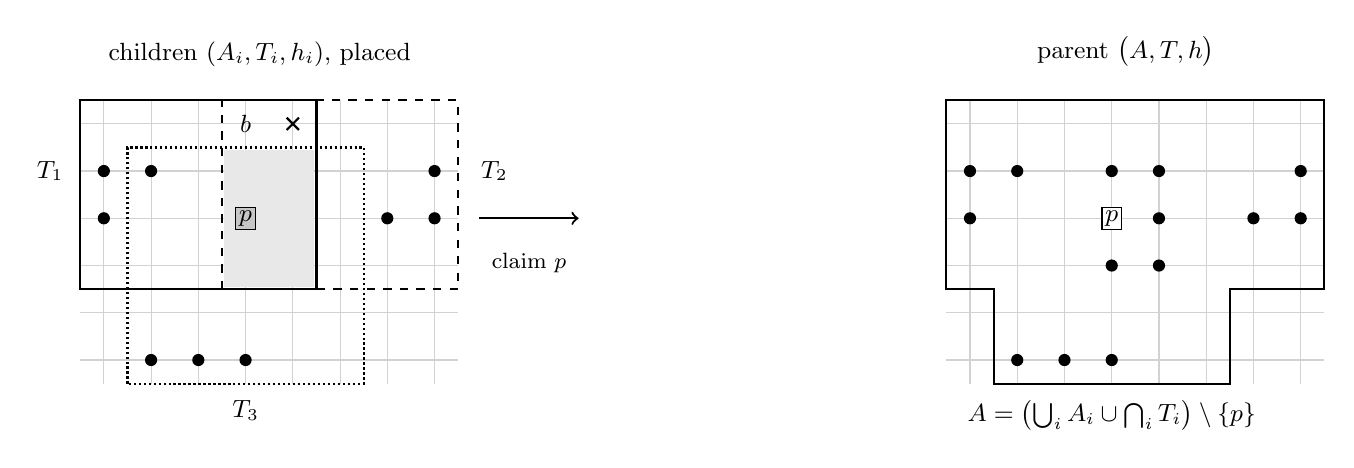
\begin{tikzpicture}[x=6mm,y=6mm,font=\small]
% ======================= left: three placed children ======================
\begin{scope}
 \draw[gray!35,step=1] (-4.5,-3.5) grid (3.5,2.5);
 % the three envelopes
 \draw[thick] (-4.5,-1.5) rectangle (0.5,2.5);
 \draw[thick,dashed] (-1.5,-1.5) rectangle (3.5,2.5);
 \draw[thick,densely dotted] (-3.5,-3.5) rectangle (1.5,1.5);
 % their common part
 \fill[gray!18] (-1.45,-1.45) rectangle (0.45,1.45);
 % required cells of the children
 \foreach \x/\y in {-4/0,-4/1,-3/1}{\fill (\x,\y) circle (2.2pt);}
 \foreach \x/\y in {2/0,3/0,3/1}{\fill (\x,\y) circle (2.2pt);}
 \foreach \x/\y in {-3/-3,-2/-3,-1/-3}{\fill (\x,\y) circle (2.2pt);}
 % the pivot, and one Breaker stone
 \node[draw,fill=gray!45,inner sep=1.2pt] at (-1,0) {$p$};
 \draw[thick] (-.13,1.87)--(.13,2.13) (-.13,2.13)--(.13,1.87);
 % labels
 \node[left] at (-4.65,1) {$T_1$};
 \node[right] at (3.78,1) {$T_2$};
 \node[below] at (-1,-3.65) {$T_3$};
 \node at (-1,2) {$b$};
 \node[above] at (-.7,3.0) {children $(A_i,T_i,h_i)$, placed};
\end{scope}
% ======================= right: the parent card ===========================
\begin{scope}[xshift=11cm]
 \draw[gray!35,step=1] (-4.5,-3.5) grid (3.5,2.5);
 % the envelope {p} u U T_i
 \draw[thick] (-4.5,2.5)--(-4.5,-1.5)--(-3.5,-1.5)--(-3.5,-3.5)--(1.5,-3.5)
              --(1.5,-1.5)--(3.5,-1.5)--(3.5,2.5)--cycle;
 % U A_i u (n T_i) minus the pivot
 \foreach \x/\y in {-4/0,-4/1,-3/1,2/0,3/0,3/1,-3/-3,-2/-3,-1/-3,
                    -1/-1,0/-1,-1/1,0/0,0/1}{\fill (\x,\y) circle (2.2pt);}
 \node[draw,fill=white,inner sep=1.2pt] at (-1,0) {$p$};
 \node[above] at (-.7,3.0) {parent $\bigl(A,T,h\bigr)$};
 \node[below] at (-1,-3.65) {$A=\bigl(\bigcup_iA_i\cup\bigcap_iT_i\bigr)\setminus\{p\}$};
\end{scope}
\draw[->,thick] (3.95,0)--(6.05,0);
\node[font=\footnotesize] at (5.0,-0.95) {claim $p$};
\end{tikzpicture}
\caption{The combination rule, Lemma~3 of the paper. Left: the children,
placed in one frame. The shaded block is $\bigcap_iT_i$; the pivot $p$
lies in it; Section~\ref{sec:pivot} says what a pivot is. Maker claims $p$, which makes every $A_i$ and the whole shaded block
Maker's. Because $p\in T$ and $T_i\subseteq T$, Breaker owns no cell of any
$T_i$; its next stone $b$ cannot be in every envelope --- here $b\notin T_3$ ---
so at least one child is still available. Right: the parent card. Its envelope
is $\{p\}\cup\bigcup_iT_i$ and its required set is the union of the child
requirements together with the common block, with the pivot spent; its height
is $1+\max_ih_i$. Nothing is assumed about Maker cells outside
$\bigcup_iA_i\cup\bigcap_iT_i$, or about Breaker cells outside the envelope.}
\label{fig:combination}
\end{figure}


\section{Building the certificate}

The leaves are Lemma~4: for each $j<6$, the five cells $S\setminus\{s_j\}$ with
envelope $S$ and height $1$ form a valid claim --- Maker owns a copy of $\Snaky$
but for one cell, so one claim finishes it.

From there the construction is mechanical. A line of the certificate gives a card
number, a pivot coordinate in a two-character alphabet (each character is one
coordinate, $0$--$9$ then $A$--$G$), and a list of children; a child is a
reference ``$j{:}sUV$'' to an earlier card $j$ placed by the signed permutation
$s$ and the translation $UV$, or a parenthesised combination of such children in
the same frame. Card $727$ has $32$ placed children drawn from six earlier cards.
Proposition~5 records the endpoint: $728$ cards, heights at most $21$,
$p_{727}=(8,8)$, $A_{727}=\varnothing$, $|T_{727}|=251$ and
$T_{727}\subseteq\{0,\dots,16\}^2$.

Two trends run through the list, and both are necessary. Heights grow by one per
level, so a card high in the list promises a win in many moves; to be worth
anything it must keep Breaker out of a large region for that long, and its
envelope grows with it, up to the $251$ cells of card $727$. Requirements run the
other way: the higher a card sits, the less it assumes about what Maker has
already built, ending at the empty set. Figure~3 shows both.

% ---------------------------------------------------------------------------
%  Suggestion: place in Section 3, just before Proposition 5, with
%  \ref{fig:landscape} in the text.
%  Generated from the certificate by gen_tikz.py; edit that, not this.
% ---------------------------------------------------------------------------
\begin{figure}[H]
\centering
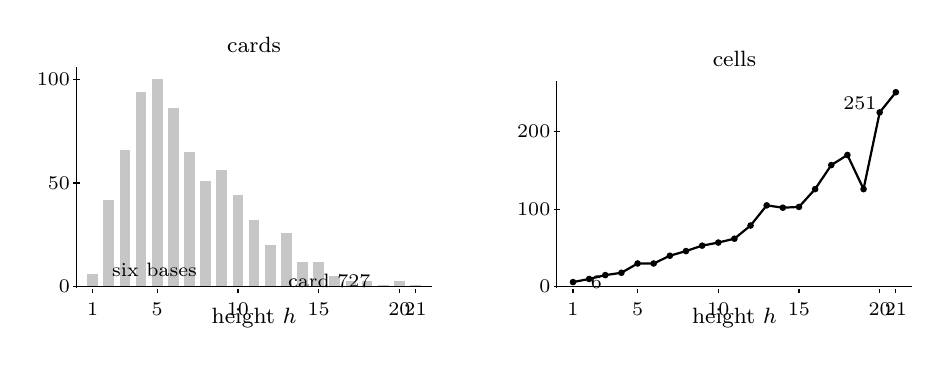
\begin{tikzpicture}[x=2.05mm,y=1pt,font=\small]
\begin{scope}
\fill[gray!45] (0.67,0) rectangle (1.33,4.50);
\fill[gray!45] (1.67,0) rectangle (2.33,31.50);
\fill[gray!45] (2.67,0) rectangle (3.33,49.50);
\fill[gray!45] (3.67,0) rectangle (4.33,70.50);
\fill[gray!45] (4.67,0) rectangle (5.33,75.00);
\fill[gray!45] (5.67,0) rectangle (6.33,64.50);
\fill[gray!45] (6.67,0) rectangle (7.33,48.75);
\fill[gray!45] (7.67,0) rectangle (8.33,38.25);
\fill[gray!45] (8.67,0) rectangle (9.33,42.00);
\fill[gray!45] (9.67,0) rectangle (10.33,33.00);
\fill[gray!45] (10.67,0) rectangle (11.33,24.00);
\fill[gray!45] (11.67,0) rectangle (12.33,15.00);
\fill[gray!45] (12.67,0) rectangle (13.33,19.50);
\fill[gray!45] (13.67,0) rectangle (14.33,9.00);
\fill[gray!45] (14.67,0) rectangle (15.33,9.00);
\fill[gray!45] (15.67,0) rectangle (16.33,3.75);
\fill[gray!45] (16.67,0) rectangle (17.33,2.25);
\fill[gray!45] (17.67,0) rectangle (18.33,2.25);
\fill[gray!45] (18.67,0) rectangle (19.33,0.75);
\fill[gray!45] (19.67,0) rectangle (20.33,2.25);
\fill[gray!45] (20.67,0) rectangle (21.33,0.75);
\draw (-.1,0)--(22,0);
\draw (0,-.5)--(0,79.50);
\draw (-.2,0.00)--(.2,0.00) node[left,font=\scriptsize] {0};
\draw (-.2,37.50)--(.2,37.50) node[left,font=\scriptsize] {50};
\draw (-.2,75.00)--(.2,75.00) node[left,font=\scriptsize] {100};
\draw (1.0,-.8)--(1.0,-2.2) node[below,font=\scriptsize] {1};
\draw (5.0,-.8)--(5.0,-2.2) node[below,font=\scriptsize] {5};
\draw (10.0,-.8)--(10.0,-2.2) node[below,font=\scriptsize] {10};
\draw (15.0,-.8)--(15.0,-2.2) node[below,font=\scriptsize] {15};
\draw (20.0,-.8)--(20.0,-2.2) node[below,font=\scriptsize] {20};
\draw (21.0,-.8)--(21.0,-2.2) node[below,font=\scriptsize] {21};
\node[below,font=\footnotesize] at (11,-4.2) {height $h$};
\node[font=\footnotesize] at (11,87.50) {cards};
\node[font=\scriptsize,anchor=west] at (1.6,6.00) {six bases};
\node[font=\scriptsize,anchor=west] at (12.5,2.25) {card $727$};
\end{scope}
\begin{scope}[xshift=6.1cm]
\draw[thick] (1.0,1.68)--(2.0,2.80)--(3.0,4.20)--(4.0,5.04)--(5.0,8.40)--(6.0,8.40)--(7.0,11.20)--(8.0,12.88)--(9.0,14.84)--(10.0,15.96)--(11.0,17.36)--(12.0,22.12)--(13.0,29.40)--(14.0,28.56)--(15.0,28.84)--(16.0,35.28)--(17.0,43.96)--(18.0,47.60)--(19.0,35.28)--(20.0,63.00)--(21.0,70.28);
\fill (1.0,1.68) circle (1.2pt);
\fill (2.0,2.80) circle (1.2pt);
\fill (3.0,4.20) circle (1.2pt);
\fill (4.0,5.04) circle (1.2pt);
\fill (5.0,8.40) circle (1.2pt);
\fill (6.0,8.40) circle (1.2pt);
\fill (7.0,11.20) circle (1.2pt);
\fill (8.0,12.88) circle (1.2pt);
\fill (9.0,14.84) circle (1.2pt);
\fill (10.0,15.96) circle (1.2pt);
\fill (11.0,17.36) circle (1.2pt);
\fill (12.0,22.12) circle (1.2pt);
\fill (13.0,29.40) circle (1.2pt);
\fill (14.0,28.56) circle (1.2pt);
\fill (15.0,28.84) circle (1.2pt);
\fill (16.0,35.28) circle (1.2pt);
\fill (17.0,43.96) circle (1.2pt);
\fill (18.0,47.60) circle (1.2pt);
\fill (19.0,35.28) circle (1.2pt);
\fill (20.0,63.00) circle (1.2pt);
\fill (21.0,70.28) circle (1.2pt);
\draw (-.1,0)--(22,0);
\draw (0,-.5)--(0,74.20);
\draw (-.2,0.00)--(.2,0.00) node[left,font=\scriptsize] {0};
\draw (-.2,28.00)--(.2,28.00) node[left,font=\scriptsize] {100};
\draw (-.2,56.00)--(.2,56.00) node[left,font=\scriptsize] {200};
\draw (1.0,-.8)--(1.0,-2.2) node[below,font=\scriptsize] {1};
\draw (5.0,-.8)--(5.0,-2.2) node[below,font=\scriptsize] {5};
\draw (10.0,-.8)--(10.0,-2.2) node[below,font=\scriptsize] {10};
\draw (15.0,-.8)--(15.0,-2.2) node[below,font=\scriptsize] {15};
\draw (20.0,-.8)--(20.0,-2.2) node[below,font=\scriptsize] {20};
\draw (21.0,-.8)--(21.0,-2.2) node[below,font=\scriptsize] {21};
\node[below,font=\footnotesize] at (11,-4.2) {height $h$};
\node[font=\footnotesize] at (11,82.20) {cells};
\node[font=\scriptsize,anchor=west] at (1.5,1.68) {$6$};
\node[font=\scriptsize,anchor=east] at (20.4,66.28) {$251$};
\end{scope}
\end{tikzpicture}
\caption{The certificate as a whole. Left, the number of cards at each height: a
pyramid from the six one-hole copies to the single card $727$. Right, the largest
envelope at each height. The two trends are the reason the construction works:
the higher a card reaches, the more cells it must keep free of Breaker
($251$ at the top), while the required sets move the other way and end empty.}
\label{fig:landscape}
\end{figure}


The last line is where the construction closes, and Table~1 of the paper is its
bookkeeping. The $32$ children come in six groups of four or eight placements.
Every placed child requires exactly $(8,8)$, and the intersection of all $32$
placed envelopes is exactly $\{(8,8)\}$: the common part of the envelopes loses
$35,31,21,12,4$ cells as the groups are added, and then nothing is left. So in
\eqref{eq:combination} the union of the requirements and the intersection are the
same singleton, and deleting the pivot leaves $A_{727}=\varnothing$. Figure~4 is
Table~1 drawn.

% ---------------------------------------------------------------------------
%  Suggestion: place in Section 3, beside Table 1 (the six groups of children
%  of card 727), with \ref{fig:topcard} in the paragraph before it.
%  Generated from the certificate by gen_tikz.py; edit that, not this.
% ---------------------------------------------------------------------------
\begin{figure}[H]
\centering
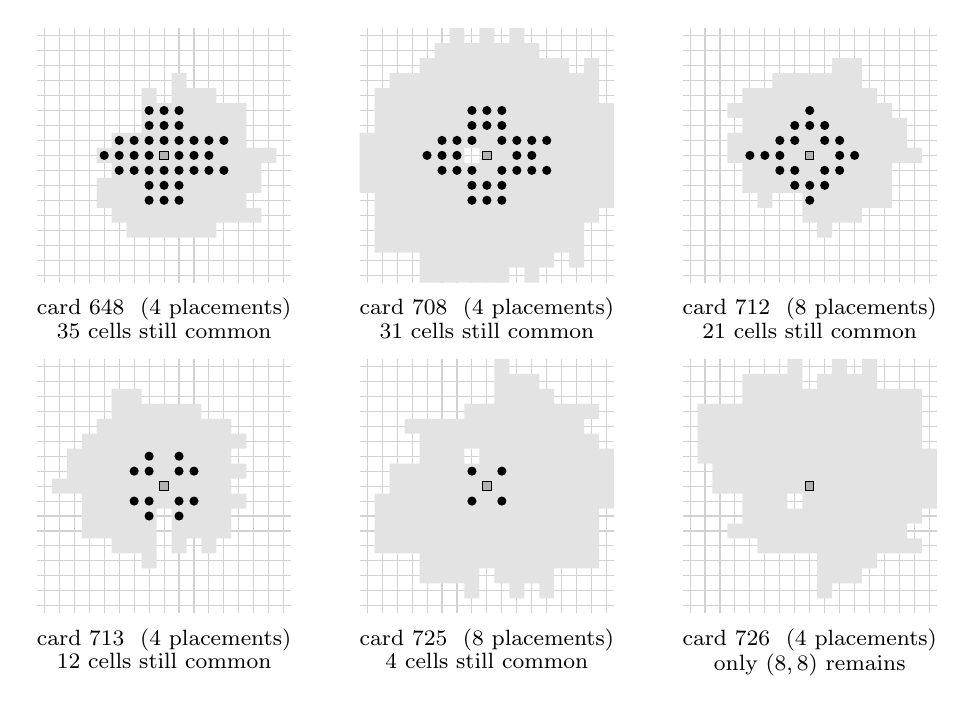
\begin{tikzpicture}[x=1.9mm,y=1.9mm,font=\small]
\begin{scope}[xshift=0.0cm,yshift=0.0cm]
\draw[gray!35,step=1] (-.5,-.5) grid (16.5,16.5);
\fill[gray!22] \foreach \x/\y in {6/3,7/3,8/3,9/3,10/3,11/3,5/4,6/4,7/4,8/4,9/4,10/4,11/4,12/4,13/4,14/4,4/5,5/5,6/5,7/5,8/5,9/5,10/5,11/5,12/5,13/5,4/6,5/6,6/6,7/6,8/6,9/6,10/6,11/6,12/6,13/6,14/6,5/7,6/7,7/7,8/7,9/7,10/7,11/7,12/7,13/7,14/7,4/8,5/8,6/8,7/8,8/8,9/8,10/8,11/8,12/8,13/8,14/8,15/8,5/9,6/9,7/9,8/9,9/9,10/9,11/9,12/9,13/9,7/10,8/10,9/10,10/10,11/10,12/10,13/10,7/11,8/11,9/11,10/11,11/11,12/11,13/11,7/12,9/12,10/12,11/12,9/13}{(\x-.5,\y-.5) rectangle (\x+.5,\y+.5)};
\fill \foreach \x/\y in {7/5,8/5,9/5,7/6,8/6,9/6,5/7,6/7,7/7,8/7,9/7,10/7,11/7,12/7,4/8,5/8,6/8,7/8,9/8,10/8,11/8,5/9,6/9,7/9,8/9,9/9,10/9,11/9,12/9,7/10,8/10,9/10,7/11,8/11,9/11}{(\x,\y) circle (.58mm)};
\filldraw[fill=gray!60] (7.72,7.72) rectangle (8.28,8.28);
\node[below,font=\footnotesize] at (8,-.9) {card 648 \ (4 placements)};
\node[below,font=\footnotesize,yshift=-3.1mm] at (8,-.9) {$35$ cells still common};
\end{scope}
\begin{scope}[xshift=4.1cm,yshift=0.0cm]
\draw[gray!35,step=1] (-.5,-.5) grid (16.5,16.5);
\fill[gray!22] \foreach \x/\y in {4/0,5/0,6/0,7/0,8/0,9/0,11/0,4/1,5/1,6/1,7/1,8/1,9/1,10/1,11/1,12/1,14/1,1/2,2/2,3/2,4/2,5/2,6/2,7/2,8/2,9/2,10/2,11/2,12/2,13/2,14/2,1/3,2/3,3/3,4/3,5/3,6/3,7/3,8/3,9/3,10/3,11/3,12/3,13/3,14/3,1/4,2/4,3/4,4/4,5/4,6/4,7/4,8/4,9/4,10/4,11/4,12/4,13/4,14/4,15/4,1/5,2/5,3/5,4/5,5/5,6/5,7/5,8/5,9/5,10/5,11/5,12/5,13/5,14/5,15/5,16/5,0/6,1/6,2/6,3/6,4/6,5/6,6/6,7/6,8/6,9/6,10/6,11/6,12/6,13/6,14/6,15/6,16/6,0/7,1/7,2/7,3/7,4/7,5/7,6/7,7/7,8/7,9/7,10/7,11/7,12/7,13/7,14/7,15/7,16/7,0/8,1/8,2/8,3/8,4/8,5/8,6/8,8/8,9/8,10/8,11/8,12/8,13/8,14/8,15/8,16/8,0/9,1/9,2/9,3/9,4/9,5/9,6/9,7/9,8/9,9/9,10/9,11/9,12/9,13/9,14/9,15/9,16/9,1/10,2/10,3/10,4/10,5/10,6/10,7/10,8/10,9/10,10/10,11/10,12/10,13/10,14/10,15/10,16/10,1/11,2/11,3/11,4/11,5/11,6/11,7/11,8/11,9/11,10/11,11/11,12/11,13/11,14/11,15/11,16/11,1/12,2/12,3/12,4/12,5/12,6/12,7/12,8/12,9/12,10/12,11/12,12/12,13/12,14/12,15/12,2/13,3/13,4/13,5/13,6/13,7/13,8/13,9/13,10/13,11/13,12/13,13/13,14/13,15/13,4/14,5/14,6/14,7/14,8/14,9/14,10/14,11/14,12/14,13/14,15/14,5/15,6/15,7/15,8/15,9/15,10/15,11/15,6/16,8/16,10/16}{(\x-.5,\y-.5) rectangle (\x+.5,\y+.5)};
\fill \foreach \x/\y in {7/5,8/5,9/5,7/6,8/6,9/6,5/7,6/7,7/7,9/7,10/7,11/7,12/7,4/8,5/8,6/8,10/8,11/8,5/9,6/9,7/9,9/9,10/9,11/9,12/9,7/10,8/10,9/10,7/11,8/11,9/11}{(\x,\y) circle (.58mm)};
\filldraw[fill=gray!60] (7.72,7.72) rectangle (8.28,8.28);
\node[below,font=\footnotesize] at (8,-.9) {card 708 \ (4 placements)};
\node[below,font=\footnotesize,yshift=-3.1mm] at (8,-.9) {$31$ cells still common};
\end{scope}
\begin{scope}[xshift=8.2cm,yshift=0.0cm]
\draw[gray!35,step=1] (-.5,-.5) grid (16.5,16.5);
\fill[gray!22] \foreach \x/\y in {9/3,8/4,9/4,10/4,11/4,5/5,8/5,9/5,10/5,11/5,12/5,13/5,4/6,5/6,6/6,7/6,8/6,9/6,10/6,11/6,12/6,13/6,4/7,5/7,6/7,7/7,8/7,9/7,10/7,11/7,12/7,13/7,3/8,4/8,5/8,6/8,7/8,8/8,9/8,10/8,11/8,12/8,13/8,14/8,15/8,3/9,4/9,5/9,6/9,7/9,8/9,9/9,10/9,11/9,12/9,13/9,14/9,4/10,5/10,6/10,7/10,8/10,9/10,10/10,11/10,12/10,13/10,14/10,3/11,4/11,5/11,6/11,7/11,8/11,9/11,10/11,11/11,12/11,13/11,4/12,5/12,6/12,7/12,8/12,9/12,10/12,11/12,12/12,6/13,7/13,8/13,9/13,10/13,11/13,10/14,11/14}{(\x-.5,\y-.5) rectangle (\x+.5,\y+.5)};
\fill \foreach \x/\y in {8/5,7/6,8/6,9/6,6/7,7/7,9/7,10/7,4/8,5/8,6/8,10/8,11/8,6/9,7/9,9/9,10/9,7/10,8/10,9/10,8/11}{(\x,\y) circle (.58mm)};
\filldraw[fill=gray!60] (7.72,7.72) rectangle (8.28,8.28);
\node[below,font=\footnotesize] at (8,-.9) {card 712 \ (8 placements)};
\node[below,font=\footnotesize,yshift=-3.1mm] at (8,-.9) {$21$ cells still common};
\end{scope}
\begin{scope}[xshift=0.0cm,yshift=-4.2cm]
\draw[gray!35,step=1] (-.5,-.5) grid (16.5,16.5);
\fill[gray!22] \foreach \x/\y in {7/3,5/4,6/4,7/4,9/4,11/4,3/5,4/5,5/5,6/5,7/5,9/5,10/5,11/5,12/5,3/6,4/6,5/6,6/6,7/6,9/6,10/6,11/6,12/6,3/7,4/7,5/7,6/7,7/7,8/7,9/7,10/7,11/7,12/7,13/7,1/8,2/8,3/8,4/8,5/8,6/8,7/8,8/8,9/8,10/8,11/8,12/8,2/9,3/9,4/9,5/9,6/9,7/9,8/9,9/9,10/9,11/9,12/9,13/9,2/10,3/10,4/10,5/10,6/10,7/10,8/10,9/10,10/10,11/10,12/10,3/11,4/11,5/11,6/11,7/11,8/11,9/11,10/11,11/11,12/11,13/11,4/12,5/12,6/12,7/12,8/12,9/12,10/12,11/12,12/12,5/13,6/13,7/13,8/13,9/13,10/13,5/14,6/14}{(\x-.5,\y-.5) rectangle (\x+.5,\y+.5)};
\fill \foreach \x/\y in {7/6,9/6,6/7,7/7,9/7,10/7,6/9,7/9,9/9,10/9,7/10,9/10}{(\x,\y) circle (.58mm)};
\filldraw[fill=gray!60] (7.72,7.72) rectangle (8.28,8.28);
\node[below,font=\footnotesize] at (8,-.9) {card 713 \ (4 placements)};
\node[below,font=\footnotesize,yshift=-3.1mm] at (8,-.9) {$12$ cells still common};
\end{scope}
\begin{scope}[xshift=4.1cm,yshift=-4.2cm]
\draw[gray!35,step=1] (-.5,-.5) grid (16.5,16.5);
\fill[gray!22] \foreach \x/\y in {7/1,10/1,12/1,4/2,5/2,6/2,7/2,9/2,10/2,11/2,12/2,4/3,5/3,6/3,7/3,8/3,9/3,10/3,11/3,12/3,13/3,14/3,15/3,1/4,2/4,3/4,4/4,5/4,6/4,7/4,8/4,9/4,10/4,11/4,12/4,13/4,14/4,15/4,1/5,2/5,3/5,4/5,5/5,6/5,7/5,8/5,9/5,10/5,11/5,12/5,13/5,14/5,15/5,1/6,2/6,3/6,4/6,5/6,6/6,7/6,8/6,9/6,10/6,11/6,12/6,13/6,14/6,15/6,1/7,2/7,3/7,4/7,5/7,6/7,7/7,8/7,9/7,10/7,11/7,12/7,13/7,14/7,15/7,16/7,2/8,3/8,4/8,5/8,6/8,7/8,8/8,9/8,10/8,11/8,12/8,13/8,14/8,15/8,16/8,2/9,3/9,4/9,5/9,6/9,7/9,8/9,9/9,10/9,11/9,12/9,13/9,14/9,15/9,16/9,4/10,5/10,6/10,8/10,9/10,10/10,11/10,12/10,13/10,14/10,15/10,16/10,4/11,5/11,6/11,7/11,8/11,9/11,10/11,11/11,12/11,13/11,14/11,15/11,3/12,4/12,5/12,6/12,7/12,8/12,9/12,10/12,11/12,12/12,13/12,14/12,7/13,8/13,9/13,10/13,11/13,12/13,13/13,14/13,15/13,9/14,10/14,11/14,12/14,9/15,10/15,11/15,9/16}{(\x-.5,\y-.5) rectangle (\x+.5,\y+.5)};
\fill \foreach \x/\y in {7/7,9/7,7/9,9/9}{(\x,\y) circle (.58mm)};
\filldraw[fill=gray!60] (7.72,7.72) rectangle (8.28,8.28);
\node[below,font=\footnotesize] at (8,-.9) {card 725 \ (8 placements)};
\node[below,font=\footnotesize,yshift=-3.1mm] at (8,-.9) {$4$ cells still common};
\end{scope}
\begin{scope}[xshift=8.2cm,yshift=-4.2cm]
\draw[gray!35,step=1] (-.5,-.5) grid (16.5,16.5);
\fill[gray!22] \foreach \x/\y in {9/1,9/2,10/2,11/2,9/3,10/3,11/3,12/3,5/4,6/4,7/4,8/4,9/4,10/4,11/4,12/4,13/4,14/4,15/4,3/5,4/5,5/5,6/5,7/5,8/5,9/5,10/5,11/5,12/5,13/5,14/5,4/6,5/6,6/6,7/6,8/6,9/6,10/6,11/6,12/6,13/6,14/6,15/6,4/7,5/7,6/7,8/7,9/7,10/7,11/7,12/7,13/7,14/7,15/7,16/7,2/8,3/8,4/8,5/8,6/8,7/8,8/8,9/8,10/8,11/8,12/8,13/8,14/8,15/8,16/8,2/9,3/9,4/9,5/9,6/9,7/9,8/9,9/9,10/9,11/9,12/9,13/9,14/9,15/9,16/9,1/10,2/10,3/10,4/10,5/10,6/10,7/10,8/10,9/10,10/10,11/10,12/10,13/10,14/10,15/10,16/10,1/11,2/11,3/11,4/11,5/11,6/11,7/11,8/11,9/11,10/11,11/11,12/11,13/11,14/11,15/11,1/12,2/12,3/12,4/12,5/12,6/12,7/12,8/12,9/12,10/12,11/12,12/12,13/12,14/12,15/12,1/13,2/13,3/13,4/13,5/13,6/13,7/13,8/13,9/13,10/13,11/13,12/13,13/13,14/13,15/13,4/14,5/14,6/14,7/14,8/14,9/14,10/14,11/14,12/14,13/14,14/14,15/14,4/15,5/15,6/15,7/15,9/15,10/15,11/15,12/15,7/16,10/16,12/16}{(\x-.5,\y-.5) rectangle (\x+.5,\y+.5)};
% no cell other than $(8,8)$ is still common
\filldraw[fill=gray!60] (7.72,7.72) rectangle (8.28,8.28);
\node[below,font=\footnotesize] at (8,-.9) {card 726 \ (4 placements)};
\node[below,font=\footnotesize,yshift=-3.1mm] at (8,-.9) {only $(8,8)$ remains};
\end{scope}
\end{tikzpicture}
\caption{The $32$ children of card $727$, grouped by the card they come from;
the card number and the number of its placements are printed below each panel.
Light cells are one placed envelope of the group. The black dots are the cells
still common to every envelope listed up to and including that group, apart from
the pivot $(8,8)$ itself, which is drawn as a grey square throughout: $35,31,21,
12,4$ and finally $0$ of them. So the intersection of all $32$ envelopes is
exactly $\{(8,8)\}$, and Maker's claim there leaves nothing to require ---
$A_{727}=\varnothing$.}
\label{fig:topcard}
\end{figure}


\section{Playing it}

Turning the certificate into a policy (Section~4 of the paper) needs two arbitrary
choices, both fixed before play: an enumeration of the board, and the printed
order of every child list. The policy then reads: at the active card, claim its
placed pivot $F(p)$; if Maker already owns it, claim the first free cell of the
enumeration instead; stop the moment a copy is complete. After Breaker's reply,
move to the first child whose placed envelope avoids that cell --- Lemma~3
guarantees one exists --- and remember the new placement $F\circ G$ if the child
was a reference.

Each non-terminal step spends exactly one Maker claim and strictly lowers the
height, so play ends within $21$ claims; and since the active card is recovered by
replaying the prescribed choices, the policy is a single function of the history,
determined without seeing any future move. That is the $\exists\sigma\forall\beta$
form: extend the policy past a win by fresh moves, and the Maker set after claim
$21$ contains a copy whenever the first $20$ Breaker replies were legal.

% ---------------------------------------------------------------------------
%  Suggestion: place in Section 4, where the descent is described
%  ("Proof of Theorem 1"), with \ref{fig:descent} in the text.
%  Generated from the certificate by gen_tikz.py; edit that, not this.
% ---------------------------------------------------------------------------
\begin{figure}[H]
\centering
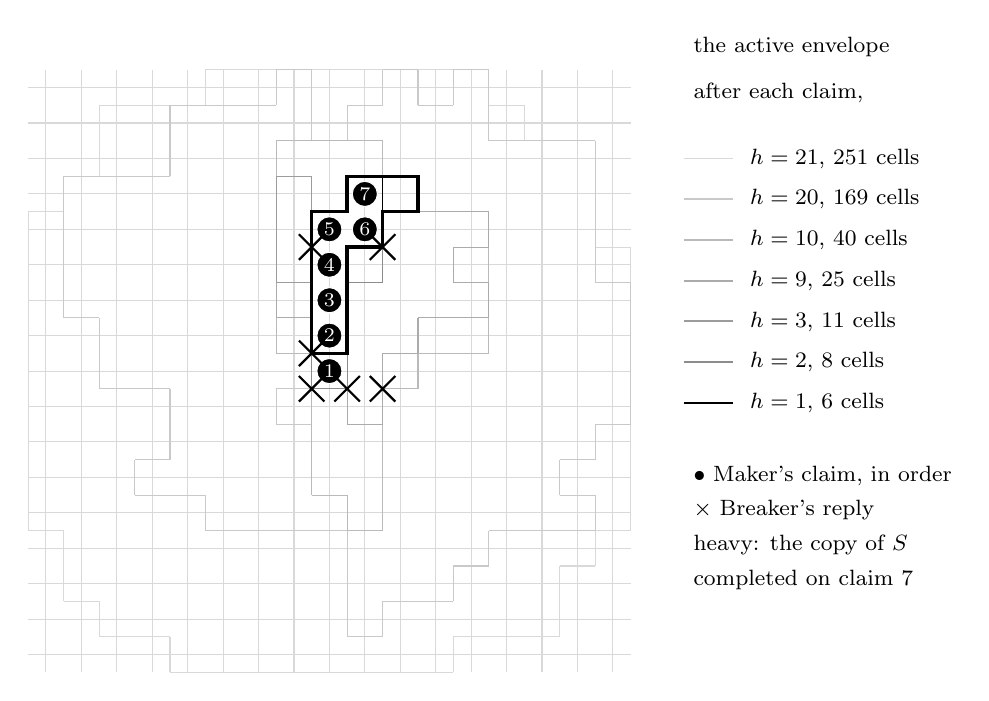
\begin{tikzpicture}[x=4.5mm,y=4.5mm,font=\small]
\draw[gray!30,step=1] (-.5,-.5) grid (16.5,16.5);
\draw[gray!30] (-0.5,3.5)--(0.5,3.5) (-0.5,3.5)--(-0.5,4.5) (-0.5,4.5)--(-0.5,5.5) (-0.5,5.5)--(-0.5,6.5) (-0.5,6.5)--(-0.5,7.5) (-0.5,7.5)--(-0.5,8.5) (-0.5,8.5)--(-0.5,9.5) (-0.5,9.5)--(-0.5,10.5) (-0.5,10.5)--(-0.5,11.5) (-0.5,12.5)--(0.5,12.5) (-0.5,11.5)--(-0.5,12.5) (0.5,1.5)--(1.5,1.5) (0.5,1.5)--(0.5,2.5) (0.5,2.5)--(0.5,3.5) (0.5,13.5)--(1.5,13.5) (0.5,12.5)--(0.5,13.5) (1.5,0.5)--(2.5,0.5) (1.5,0.5)--(1.5,1.5) (1.5,13.5)--(1.5,14.5) (1.5,15.5)--(2.5,15.5) (1.5,14.5)--(1.5,15.5) (2.5,0.5)--(3.5,0.5) (2.5,15.5)--(3.5,15.5) (3.5,-0.5)--(4.5,-0.5) (3.5,-0.5)--(3.5,0.5) (3.5,15.5)--(4.5,15.5) (4.5,-0.5)--(5.5,-0.5) (4.5,16.5)--(5.5,16.5) (4.5,15.5)--(4.5,16.5) (5.5,-0.5)--(6.5,-0.5) (5.5,16.5)--(6.5,16.5) (6.5,-0.5)--(7.5,-0.5) (6.5,16.5)--(7.5,16.5) (7.5,-0.5)--(8.5,-0.5) (7.5,16.5)--(8.5,16.5) (8.5,-0.5)--(9.5,-0.5) (8.5,16.5)--(9.5,16.5) (9.5,-0.5)--(10.5,-0.5) (9.5,16.5)--(10.5,16.5) (10.5,-0.5)--(11.5,-0.5) (11.5,-0.5)--(11.5,0.5) (10.5,16.5)--(11.5,16.5) (11.5,0.5)--(12.5,0.5) (11.5,16.5)--(12.5,16.5) (12.5,15.5)--(12.5,16.5) (12.5,0.5)--(13.5,0.5) (12.5,15.5)--(13.5,15.5) (13.5,14.5)--(13.5,15.5) (13.5,0.5)--(14.5,0.5) (14.5,0.5)--(14.5,1.5) (14.5,1.5)--(14.5,2.5) (13.5,14.5)--(14.5,14.5) (14.5,2.5)--(15.5,2.5) (15.5,2.5)--(15.5,3.5) (15.5,11.5)--(15.5,12.5) (15.5,12.5)--(15.5,13.5) (14.5,14.5)--(15.5,14.5) (15.5,13.5)--(15.5,14.5) (15.5,3.5)--(16.5,3.5) (16.5,3.5)--(16.5,4.5) (16.5,4.5)--(16.5,5.5) (16.5,5.5)--(16.5,6.5) (16.5,6.5)--(16.5,7.5) (16.5,7.5)--(16.5,8.5) (16.5,8.5)--(16.5,9.5) (16.5,9.5)--(16.5,10.5) (15.5,11.5)--(16.5,11.5) (16.5,10.5)--(16.5,11.5);
\draw[gray!42] (0.5,9.5)--(1.5,9.5) (0.5,9.5)--(0.5,10.5) (0.5,10.5)--(0.5,11.5) (0.5,11.5)--(0.5,12.5) (0.5,13.5)--(1.5,13.5) (0.5,12.5)--(0.5,13.5) (1.5,7.5)--(2.5,7.5) (1.5,7.5)--(1.5,8.5) (1.5,8.5)--(1.5,9.5) (1.5,13.5)--(2.5,13.5) (2.5,5.5)--(3.5,5.5) (2.5,4.5)--(3.5,4.5) (2.5,4.5)--(2.5,5.5) (2.5,7.5)--(3.5,7.5) (2.5,13.5)--(3.5,13.5) (3.5,4.5)--(4.5,4.5) (3.5,5.5)--(3.5,6.5) (3.5,6.5)--(3.5,7.5) (3.5,13.5)--(3.5,14.5) (3.5,15.5)--(4.5,15.5) (3.5,14.5)--(3.5,15.5) (4.5,3.5)--(5.5,3.5) (4.5,3.5)--(4.5,4.5) (4.5,15.5)--(5.5,15.5) (5.5,3.5)--(6.5,3.5) (6.5,6.5)--(6.5,7.5) (5.5,15.5)--(6.5,15.5) (6.5,3.5)--(7.5,3.5) (6.5,6.5)--(7.5,6.5) (6.5,7.5)--(7.5,7.5) (7.5,14.5)--(7.5,15.5) (6.5,16.5)--(7.5,16.5) (6.5,15.5)--(6.5,16.5) (7.5,15.5)--(7.5,16.5) (7.5,3.5)--(8.5,3.5) (7.5,6.5)--(7.5,7.5) (7.5,14.5)--(8.5,14.5) (8.5,0.5)--(9.5,0.5) (8.5,0.5)--(8.5,1.5) (9.5,0.5)--(9.5,1.5) (8.5,1.5)--(8.5,2.5) (8.5,2.5)--(8.5,3.5) (8.5,15.5)--(9.5,15.5) (8.5,14.5)--(8.5,15.5) (9.5,1.5)--(10.5,1.5) (9.5,16.5)--(10.5,16.5) (9.5,15.5)--(9.5,16.5) (10.5,15.5)--(10.5,16.5) (10.5,1.5)--(11.5,1.5) (11.5,1.5)--(11.5,2.5) (10.5,15.5)--(11.5,15.5) (11.5,2.5)--(12.5,2.5) (12.5,2.5)--(12.5,3.5) (12.5,14.5)--(12.5,15.5) (11.5,16.5)--(12.5,16.5) (11.5,15.5)--(11.5,16.5) (12.5,15.5)--(12.5,16.5) (12.5,3.5)--(13.5,3.5) (12.5,14.5)--(13.5,14.5) (13.5,3.5)--(14.5,3.5) (14.5,4.5)--(14.5,5.5) (13.5,14.5)--(14.5,14.5) (14.5,4.5)--(15.5,4.5) (14.5,3.5)--(15.5,3.5) (15.5,3.5)--(15.5,4.5) (14.5,5.5)--(15.5,5.5) (15.5,5.5)--(15.5,6.5) (15.5,10.5)--(15.5,11.5) (15.5,11.5)--(15.5,12.5) (15.5,12.5)--(15.5,13.5) (14.5,14.5)--(15.5,14.5) (15.5,13.5)--(15.5,14.5) (15.5,6.5)--(16.5,6.5) (16.5,6.5)--(16.5,7.5) (16.5,7.5)--(16.5,8.5) (16.5,8.5)--(16.5,9.5) (15.5,10.5)--(16.5,10.5) (16.5,9.5)--(16.5,10.5);
\draw[gray!54] (6.5,8.5)--(7.5,8.5) (6.5,8.5)--(6.5,9.5) (6.5,9.5)--(6.5,10.5) (6.5,10.5)--(6.5,11.5) (6.5,11.5)--(6.5,12.5) (6.5,12.5)--(6.5,13.5) (6.5,14.5)--(7.5,14.5) (6.5,13.5)--(6.5,14.5) (7.5,4.5)--(8.5,4.5) (7.5,4.5)--(7.5,5.5) (7.5,5.5)--(7.5,6.5) (7.5,6.5)--(7.5,7.5) (7.5,7.5)--(7.5,8.5) (7.5,14.5)--(8.5,14.5) (8.5,3.5)--(9.5,3.5) (8.5,3.5)--(8.5,4.5) (9.5,3.5)--(9.5,4.5) (9.5,4.5)--(9.5,5.5) (9.5,5.5)--(9.5,6.5) (9.5,6.5)--(9.5,7.5) (9.5,12.5)--(9.5,13.5) (8.5,14.5)--(9.5,14.5) (9.5,13.5)--(9.5,14.5) (9.5,7.5)--(10.5,7.5) (10.5,7.5)--(10.5,8.5) (9.5,12.5)--(10.5,12.5) (10.5,8.5)--(11.5,8.5) (10.5,12.5)--(11.5,12.5) (11.5,8.5)--(12.5,8.5) (12.5,8.5)--(12.5,9.5) (12.5,9.5)--(12.5,10.5) (12.5,10.5)--(12.5,11.5) (11.5,12.5)--(12.5,12.5) (12.5,11.5)--(12.5,12.5);
\draw[gray!66] (6.5,9.5)--(7.5,9.5) (6.5,9.5)--(6.5,10.5) (6.5,10.5)--(6.5,11.5) (6.5,11.5)--(6.5,12.5) (6.5,13.5)--(7.5,13.5) (6.5,12.5)--(6.5,13.5) (7.5,12.5)--(7.5,13.5) (7.5,7.5)--(8.5,7.5) (7.5,7.5)--(7.5,8.5) (7.5,8.5)--(7.5,9.5) (7.5,12.5)--(8.5,12.5) (8.5,6.5)--(9.5,6.5) (8.5,6.5)--(8.5,7.5) (9.5,6.5)--(9.5,7.5) (9.5,7.5)--(9.5,8.5) (8.5,13.5)--(9.5,13.5) (8.5,12.5)--(8.5,13.5) (9.5,12.5)--(9.5,13.5) (9.5,8.5)--(10.5,8.5) (10.5,8.5)--(10.5,9.5) (9.5,12.5)--(10.5,12.5) (10.5,9.5)--(11.5,9.5) (11.5,10.5)--(11.5,11.5) (10.5,12.5)--(11.5,12.5) (11.5,10.5)--(12.5,10.5) (11.5,9.5)--(12.5,9.5) (12.5,9.5)--(12.5,10.5) (11.5,12.5)--(12.5,12.5) (11.5,11.5)--(12.5,11.5) (12.5,11.5)--(12.5,12.5);
\draw[gray!78] (6.5,10.5)--(7.5,10.5) (6.5,10.5)--(6.5,11.5) (6.5,11.5)--(6.5,12.5) (6.5,13.5)--(7.5,13.5) (6.5,12.5)--(6.5,13.5) (7.5,12.5)--(7.5,13.5) (7.5,7.5)--(8.5,7.5) (7.5,7.5)--(7.5,8.5) (8.5,7.5)--(8.5,8.5) (7.5,8.5)--(7.5,9.5) (8.5,8.5)--(8.5,9.5) (7.5,9.5)--(7.5,10.5) (8.5,9.5)--(8.5,10.5) (7.5,12.5)--(8.5,12.5) (8.5,10.5)--(9.5,10.5) (9.5,10.5)--(9.5,11.5) (9.5,11.5)--(9.5,12.5) (8.5,13.5)--(9.5,13.5) (8.5,12.5)--(8.5,13.5) (9.5,12.5)--(9.5,13.5);
\draw[gray!90] (7.5,7.5)--(8.5,7.5) (7.5,7.5)--(7.5,8.5) (8.5,7.5)--(8.5,8.5) (7.5,8.5)--(7.5,9.5) (8.5,8.5)--(8.5,9.5) (7.5,9.5)--(7.5,10.5) (8.5,9.5)--(8.5,10.5) (7.5,10.5)--(7.5,11.5) (7.5,12.5)--(8.5,12.5) (7.5,11.5)--(7.5,12.5) (8.5,10.5)--(9.5,10.5) (9.5,10.5)--(9.5,11.5) (9.5,11.5)--(9.5,12.5) (8.5,13.5)--(9.5,13.5) (8.5,12.5)--(8.5,13.5) (9.5,12.5)--(9.5,13.5);
\draw[black] (7.5,8.5)--(8.5,8.5) (7.5,8.5)--(7.5,9.5) (8.5,8.5)--(8.5,9.5) (7.5,9.5)--(7.5,10.5) (8.5,9.5)--(8.5,10.5) (7.5,10.5)--(7.5,11.5) (8.5,10.5)--(8.5,11.5) (7.5,12.5)--(8.5,12.5) (7.5,11.5)--(7.5,12.5) (8.5,11.5)--(9.5,11.5) (9.5,11.5)--(9.5,12.5) (8.5,13.5)--(9.5,13.5) (8.5,12.5)--(8.5,13.5) (9.5,12.5)--(9.5,13.5);
\draw[very thick] (7.5,8.5)--(8.5,8.5)--(8.5,11.5)--(9.5,11.5)--(9.5,12.5)--(10.5,12.5)--(10.5,13.5)--(8.5,13.5)--(8.5,12.5)--(7.5,12.5)--cycle;
\node[circle,fill=black,text=white,inner sep=0pt,minimum size=3.2mm,font=\scriptsize,draw=white,line width=.4pt] at (8,8) {1};
\node[circle,fill=black,text=white,inner sep=0pt,minimum size=3.2mm,font=\scriptsize,draw=white,line width=.4pt] at (8,9) {2};
\node[circle,fill=black,text=white,inner sep=0pt,minimum size=3.2mm,font=\scriptsize,draw=white,line width=.4pt] at (8,10) {3};
\node[circle,fill=black,text=white,inner sep=0pt,minimum size=3.2mm,font=\scriptsize,draw=white,line width=.4pt] at (8,11) {4};
\node[circle,fill=black,text=white,inner sep=0pt,minimum size=3.2mm,font=\scriptsize,draw=white,line width=.4pt] at (8,12) {5};
\node[circle,fill=black,text=white,inner sep=0pt,minimum size=3.2mm,font=\scriptsize,draw=white,line width=.4pt] at (9,12) {6};
\node[circle,fill=black,text=white,inner sep=0pt,minimum size=3.2mm,font=\scriptsize,draw=white,line width=.4pt] at (9,13) {7};
\draw[thick] (7.14,7.14)--(7.86,7.86) (7.14,7.86)--(7.86,7.14);
\draw[thick] (7.14,8.14)--(7.86,8.86) (7.14,8.86)--(7.86,8.14);
\draw[thick] (8.14,7.14)--(8.86,7.86) (8.14,7.86)--(8.86,7.14);
\draw[thick] (9.14,7.14)--(9.86,7.86) (9.14,7.86)--(9.86,7.14);
\draw[thick] (7.14,11.14)--(7.86,11.86) (7.14,11.86)--(7.86,11.14);
\draw[thick] (9.14,11.14)--(9.86,11.86) (9.14,11.86)--(9.86,11.14);
\node[anchor=south west,font=\footnotesize] at (18.0,16.6) {the active envelope};
\node[anchor=south west,font=\footnotesize] at (18.0,15.3) {after each claim,};
\draw[gray!30,line width=.7pt] (18.0,14)--(19.4,14);\node[right,font=\footnotesize] at (19.6,14) {$h=21$, 251 cells};
\draw[gray!42,line width=.7pt] (18.0,12.85)--(19.4,12.85);\node[right,font=\footnotesize] at (19.6,12.85) {$h=20$, 169 cells};
\draw[gray!54,line width=.7pt] (18.0,11.7)--(19.4,11.7);\node[right,font=\footnotesize] at (19.6,11.7) {$h=10$, 40 cells};
\draw[gray!66,line width=.7pt] (18.0,10.55)--(19.4,10.55);\node[right,font=\footnotesize] at (19.6,10.55) {$h=9$, 25 cells};
\draw[gray!78,line width=.7pt] (18.0,9.4)--(19.4,9.4);\node[right,font=\footnotesize] at (19.6,9.4) {$h=3$, 11 cells};
\draw[gray!90,line width=.7pt] (18.0,8.25)--(19.4,8.25);\node[right,font=\footnotesize] at (19.6,8.25) {$h=2$, 8 cells};
\draw[black,line width=.7pt] (18.0,7.1)--(19.4,7.1);\node[right,font=\footnotesize] at (19.6,7.1) {$h=1$, 6 cells};
\node[anchor=north west,font=\footnotesize,align=left] at (18.0,5.6)
 {$\bullet$\ Maker's claim, in order\\[3pt]$\times$\ Breaker's reply\\[3pt]
  heavy: the copy of $S$\\[3pt] completed on claim $7$};
\end{tikzpicture}
\caption{One play of the policy of Section~\ref{sec:strategy}, against a Breaker
that always blocks as many child envelopes as possible. The numbered dots are Maker's
claims, each the pivot of the card then active; the crosses are Breaker's replies.
The outlines, progressively darker, are the active envelope after each claim ---
$251,169,40,25,11,8$ and $6$ cells, with heights $21,20,10,9,3,2$ and $1$. Each reply
misses one of them and play descends into it. The heaviest outline is the copy of $S$ completed on claim $7$; the
remaining bound was never needed. No cell outside these regions influences the play.}
\label{fig:descent}
\end{figure}


Figure~5 is one play of exactly this policy, against a Breaker that always blocks
as many child envelopes as possible. It is worth reading with the caption: the
outer envelope is the $251$-cell board, each claim is the pivot of the card
reached, and the envelope contracts $251\to169\to40\to25\to11\to8\to6$ as the
height falls $21\to20\to10\to9\to3\to2\to1$. The copy is complete on claim $7$.

\section{What this companion does not cover}

The paper gives three complete constructions. This one --- the certificate above,
with the $21$-move bound --- is the sharpest and the one that closes with no
required cells at all; the $25$-move construction of Appendix~A records reduced
envelopes and needs an explicit opening cover for five exceptional first replies,
and the $35$-move construction of Appendix~B supplies four conditional strategies
stated at arbitrary positions. All three use the rule of Section~3 and differ in
what they carry; only the first is drawn here. Section~5 of the paper proves a
separate local statement, that four Maker stones in a row win against at most
three nearby Breaker stones, which explains the geometry behind the threats
without being needed for the bound. The appendices print the certificate data, and
the verification programs of Section~6 and Appendix~G check the finite
reconstruction.

\section{How the figures were made and checked}

None of the geometry is drawn by hand. The file
\texttt{verification/certificate.txt} distributed with the paper was checked
against the SHA-256 that Section~6.2 states, and then parsed again independently:
all $728$ cards were recomputed from Definition~2 and \eqref{eq:combination},
reproducing $|T_{727}|=251$, $h_{727}=21$ and the intermediate values of Table~1
--- including the running intersection of Figure~4, which loses
$35,31,21,12,4,0$ cells. Figures~2--5 are drawn from those recomputed sets.

Figure~5 is a simulation of the Section~4 policy, with the invariant of
Definition~2 --- Breaker owns nothing in the active envelope, Maker owns the whole
required set --- asserted at every step. Over two hundred randomised Breaker
strategies and one greedy one, every play finished in six to eight claims; the
figure shows a representative one, not the worst case.

The claim about pivots in Section~3 was checked the same way: over all $1{,}620$
combination nodes, the pivot lay in every child's required set, with no exception.
Both programs are in \texttt{code/} and need only the certificate file.


\vspace{6pt}
\begin{center}
\small
\begin{tabular}{@{}lll@{}}
\toprule
in the paper & what it does & figure here \\
\midrule
\S1 & the game, the theorem, earlier work & Figure 1 \\
\S2 & Definition 2, Lemma 3, Lemma 4 & Figures 1, 2 \\
\S3 & the certificate, Proposition 5, Table 1 & Figures 3, 4 \\
\S4 & the policy and its move count & Figure 5 \\
\S5 & four in a row, Proposition 7 & --- \\
\S6 & exact reconstruction and its scope & --- \\
App.~A, B & the 25- and 35-move constructions & --- \\
App.~D--F & the certificate data & --- \\
App.~G & the verification programs & --- \\
\bottomrule
\end{tabular}
\end{center}

\end{document}
